\begin{tikzpicture}
\node[inner sep=0pt] (obrazek) at (0,0)
    {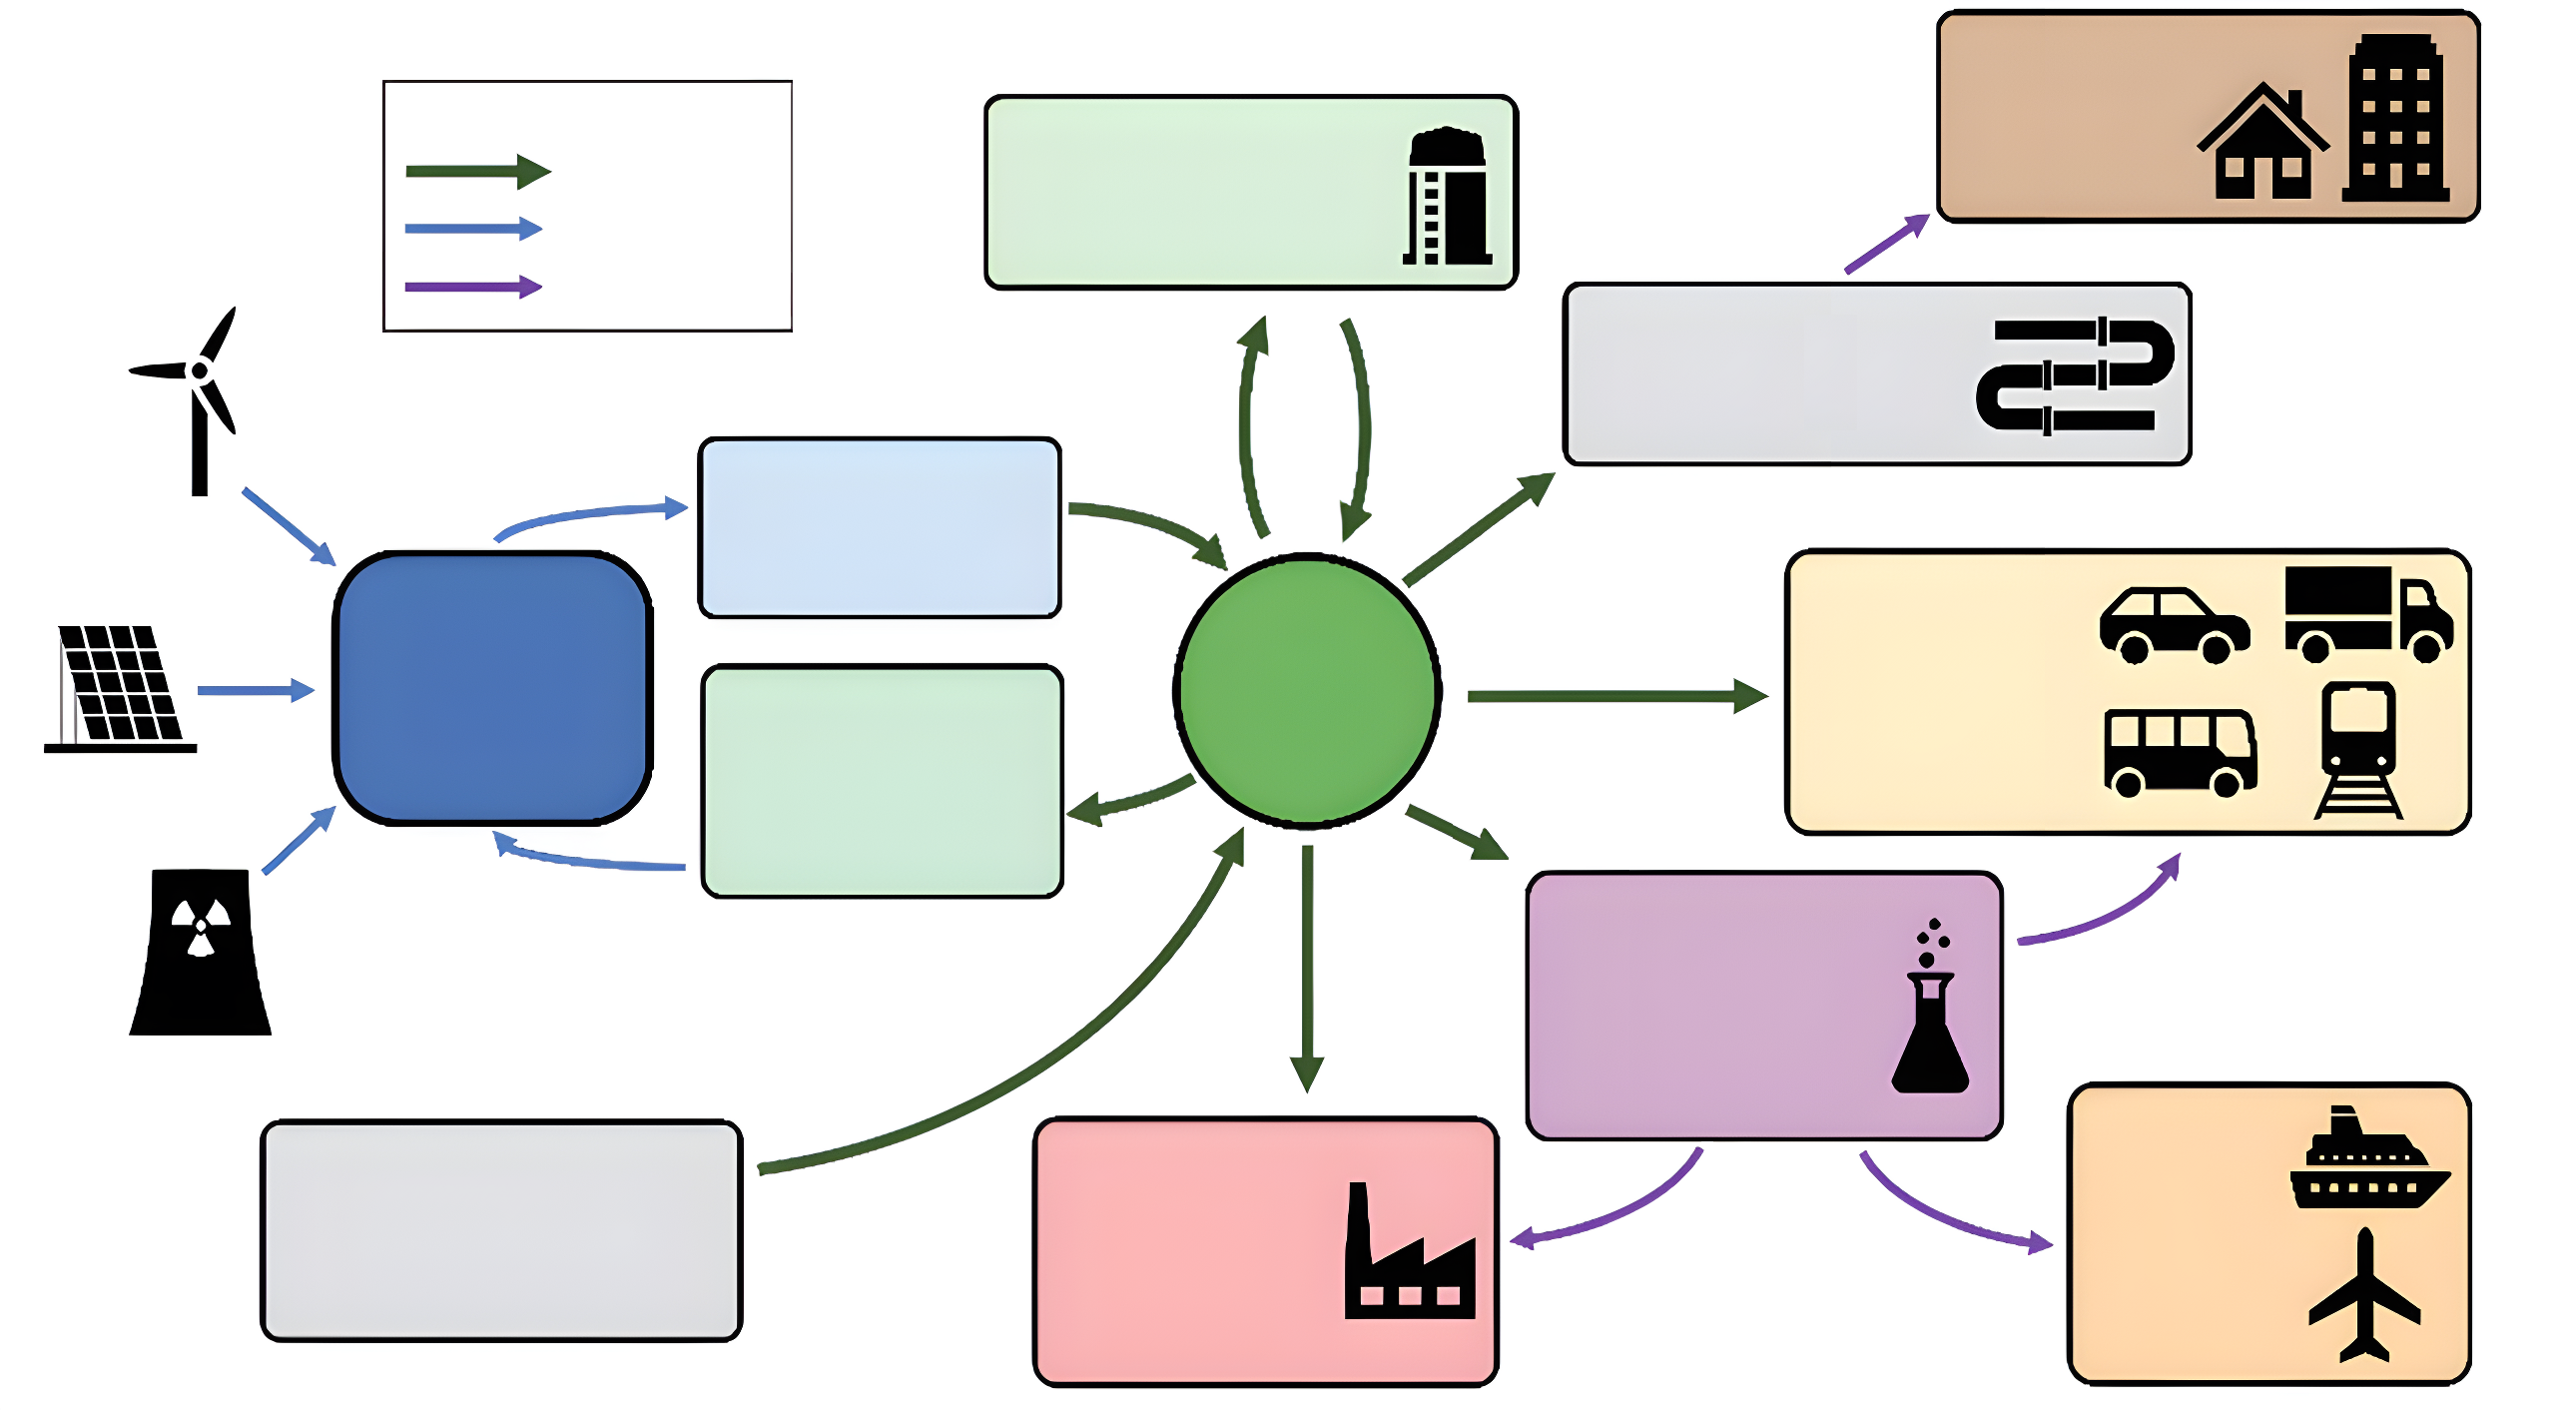
\includegraphics[width=1.01\textwidth]{figures/pouziti_vodiku.png}};
\node[font=\scriptsize] at (-3.86,3.23) {Nosiče energie};
\node[font=\scriptsize,align=left] at (-3.4,2.6) {Vodík\\Elektřina\\Ostatní};
\node[font=\scriptsize,text=white,align=center] at (-4.4,0.1) {Elektrická\\síť};
\node[font=\scriptsize,align=center] at (-2.25,1) {Výroba\\elektrolýzou};
\node[font=\scriptsize,align=center] at (-2.23,-0.4) {Palivové\\články,\\turbíny};
\node[font=\LARGE] at (0.1,0.07) {$\mathrm{H_2}$};
\node[font=\scriptsize,align=center] at (-4.3,-2.9) {Výroba\\z fosilních paliv};
\node[font=\scriptsize,align=center] at (-0.5,2.8) {\textbf{Skladování}\\tlakové nádoby,\\podzemí};
\node[font=\scriptsize,align=center] at (2.6,1.85) {\textbf{Plyn. sítě\footnotemark}\\metanizace};
\node[font=\scriptsize,align=center] at (4.3,3.25) {\textbf{Budovy}\\topení,\\vaření};
\node[font=\scriptsize,align=center] at (3.55,0.1) {\textbf{Doprava}\\osobní,\\nákladní};
\node[font=\scriptsize,align=center] at (2.38,-1.62) {\textbf{Syntéza paliv}\\metanol, \\amoniak, $\ldots$};
\node[font=\scriptsize,align=center] at (-0.52,-2.95) {\textbf{Průmysl}\\rafinace,\\chemikálie};
\node[font=\scriptsize,align=center] at (4.9,-2.85) {\textbf{Ostatní}\\\textbf{využití}\\např.\\letectví};
\end{tikzpicture}